\documentclass[14pt]{extbook}
\usepackage{multicol, enumerate, enumitem, hyperref, color, soul, setspace, parskip, fancyhdr} %General Packages
\usepackage{amssymb, amsthm, amsmath, bbm, latexsym, units, mathtools} %Math Packages
\everymath{\displaystyle} %All math in Display Style
% Packages with additional options
\usepackage[headsep=0.5cm,headheight=12pt, left=1 in,right= 1 in,top= 1 in,bottom= 1 in]{geometry}
\usepackage[usenames,dvipsnames]{xcolor}
\usepackage{dashrule}  % Package to use the command below to create lines between items
\newcommand{\litem}[1]{\item#1\hspace*{-1cm}\rule{\textwidth}{0.4pt}}
\pagestyle{fancy}
\lhead{Progress Quiz 5}
\chead{}
\rhead{Version A}
\lfoot{9912-2038}
\cfoot{}
\rfoot{Spring 2021}
\begin{document}

\begin{enumerate}
\litem{
Construct the lowest-degree polynomial given the zeros below. Then, choose the intervals that contain the coefficients of the polynomial in the form $ax^3+bx^2+cx+d$.\[ \frac{5}{4}, \frac{-1}{4}, \text{ and } \frac{-5}{2} \]\begin{enumerate}[label=\Alph*.]
\item \( a \in [31, 39], b \in [125, 129], c \in [125, 134], \text{ and } d \in [25, 29] \)
\item \( a \in [31, 39], b \in [44, 51], c \in [-91, -83], \text{ and } d \in [-30, -22] \)
\item \( a \in [31, 39], b \in [-57, -45], c \in [-91, -83], \text{ and } d \in [25, 29] \)
\item \( a \in [31, 39], b \in [111, 113], c \in [70, 76], \text{ and } d \in [-30, -22] \)
\item \( a \in [31, 39], b \in [44, 51], c \in [-91, -83], \text{ and } d \in [25, 29] \)

\end{enumerate} }
\litem{
Describe the zero behavior of the zero $x = -3$ of the polynomial below.\[ f(x) = 8(x + 3)^{3}(x - 3)^{4}(x + 8)^{2}(x - 8)^{3} \]\begin{enumerate}[label=\Alph*.]
\begin{multicols}{2}\item 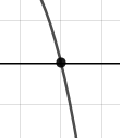
\includegraphics[width = 0.3\textwidth]{../Figures/polyZeroBehaviorAA.png}\item 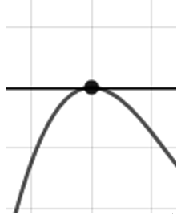
\includegraphics[width = 0.3\textwidth]{../Figures/polyZeroBehaviorBA.png}\item 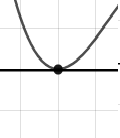
\includegraphics[width = 0.3\textwidth]{../Figures/polyZeroBehaviorCA.png}\item 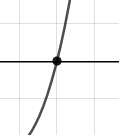
\includegraphics[width = 0.3\textwidth]{../Figures/polyZeroBehaviorDA.png}\end{multicols}\item None of the above.
\end{enumerate} }
\litem{
Describe the end behavior of the polynomial below.\[ f(x) = -4(x - 9)^{3}(x + 9)^{8}(x + 3)^{5}(x - 3)^{7} \]\begin{enumerate}[label=\Alph*.]
\begin{multicols}{2}\item 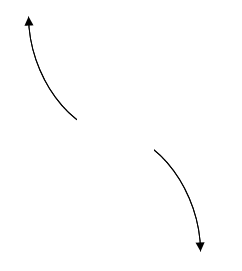
\includegraphics[width = 0.3\textwidth]{../Figures/polyEndBehaviorAA.png}\item 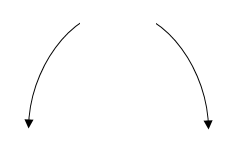
\includegraphics[width = 0.3\textwidth]{../Figures/polyEndBehaviorBA.png}\item 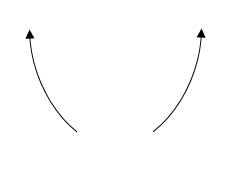
\includegraphics[width = 0.3\textwidth]{../Figures/polyEndBehaviorCA.png}\item 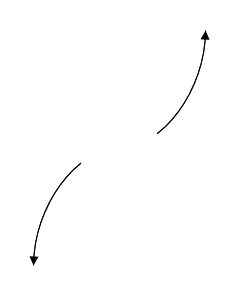
\includegraphics[width = 0.3\textwidth]{../Figures/polyEndBehaviorDA.png}\end{multicols}\item None of the above.
\end{enumerate} }
\litem{
Describe the zero behavior of the zero $x = -3$ of the polynomial below.\[ f(x) = 7(x + 2)^{8}(x - 2)^{7}(x - 3)^{11}(x + 3)^{8} \]\begin{enumerate}[label=\Alph*.]
\begin{multicols}{2}\item 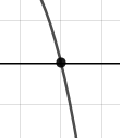
\includegraphics[width = 0.3\textwidth]{../Figures/polyZeroBehaviorCopyAA.png}\item 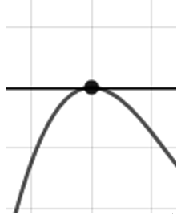
\includegraphics[width = 0.3\textwidth]{../Figures/polyZeroBehaviorCopyBA.png}\item 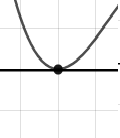
\includegraphics[width = 0.3\textwidth]{../Figures/polyZeroBehaviorCopyCA.png}\item 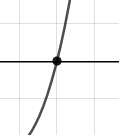
\includegraphics[width = 0.3\textwidth]{../Figures/polyZeroBehaviorCopyDA.png}\end{multicols}\item None of the above.
\end{enumerate} }
\litem{
Describe the end behavior of the polynomial below.\[ f(x) = 4(x + 6)^{2}(x - 6)^{7}(x - 8)^{5}(x + 8)^{7} \]\begin{enumerate}[label=\Alph*.]
\begin{multicols}{2}\item 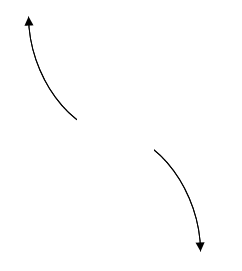
\includegraphics[width = 0.3\textwidth]{../Figures/polyEndBehaviorCopyAA.png}\item 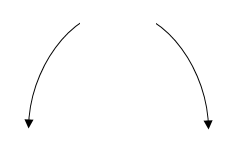
\includegraphics[width = 0.3\textwidth]{../Figures/polyEndBehaviorCopyBA.png}\item 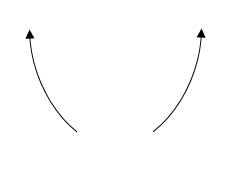
\includegraphics[width = 0.3\textwidth]{../Figures/polyEndBehaviorCopyCA.png}\item 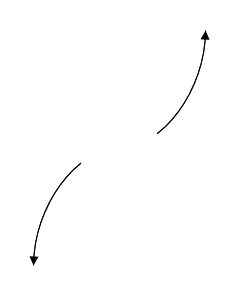
\includegraphics[width = 0.3\textwidth]{../Figures/polyEndBehaviorCopyDA.png}\end{multicols}\item None of the above.
\end{enumerate} }
\litem{
Construct the lowest-degree polynomial given the zeros below. Then, choose the intervals that contain the coefficients of the polynomial in the form $x^3+bx^2+cx+d$.\[ -3 + 2 i \text{ and } 4 \]\begin{enumerate}[label=\Alph*.]
\item \( b \in [1.3, 4.5], c \in [-12.6, -8.5], \text{ and } d \in [-54, -46] \)
\item \( b \in [-0.4, 1.2], c \in [-6.2, -5.7], \text{ and } d \in [-1, 10] \)
\item \( b \in [-0.4, 1.2], c \in [-2.3, -0.7], \text{ and } d \in [-14, -8] \)
\item \( b \in [-2.6, -1.3], c \in [-12.6, -8.5], \text{ and } d \in [48, 58] \)
\item \( \text{None of the above.} \)

\end{enumerate} }
\litem{
Construct the lowest-degree polynomial given the zeros below. Then, choose the intervals that contain the coefficients of the polynomial in the form $x^3+bx^2+cx+d$.\[ -4 + 2 i \text{ and } 1 \]\begin{enumerate}[label=\Alph*.]
\item \( b \in [-1, 5], c \in [3, 4], \text{ and } d \in [-6, -3] \)
\item \( b \in [-12, -5], c \in [6, 24], \text{ and } d \in [20, 27] \)
\item \( b \in [-1, 5], c \in [-3, 1], \text{ and } d \in [1, 6] \)
\item \( b \in [5, 11], c \in [6, 24], \text{ and } d \in [-23, -18] \)
\item \( \text{None of the above.} \)

\end{enumerate} }
\litem{
Which of the following equations \textit{could} be of the graph presented below?
\begin{center}
    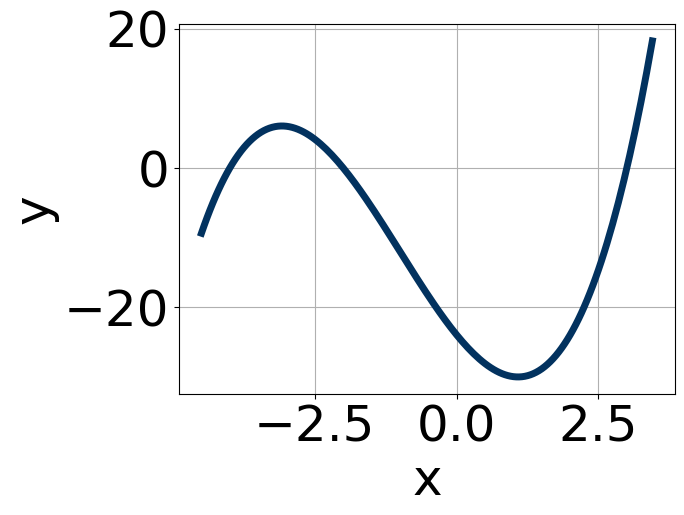
\includegraphics[width=0.5\textwidth]{../Figures/polyGraphToFunctionCopyA.png}
\end{center}
\begin{enumerate}[label=\Alph*.]
\item \( -14(x - 3)^{6} (x - 2)^{11} (x + 1)^{10} \)
\item \( 7(x - 3)^{9} (x - 2)^{6} (x + 1)^{11} \)
\item \( -7(x - 3)^{8} (x - 2)^{7} (x + 1)^{9} \)
\item \( 9(x - 3)^{6} (x - 2)^{4} (x + 1)^{11} \)
\item \( 8(x - 3)^{4} (x - 2)^{5} (x + 1)^{5} \)

\end{enumerate} }
\litem{
Construct the lowest-degree polynomial given the zeros below. Then, choose the intervals that contain the coefficients of the polynomial in the form $ax^3+bx^2+cx+d$.\[ -1, \frac{-1}{2}, \text{ and } \frac{4}{3} \]\begin{enumerate}[label=\Alph*.]
\item \( a \in [4, 11], b \in [-0.8, 1.7], c \in [-20, -8], \text{ and } d \in [-6, -2] \)
\item \( a \in [4, 11], b \in [-0.8, 1.7], c \in [-20, -8], \text{ and } d \in [3, 5] \)
\item \( a \in [4, 11], b \in [-3, -0.3], c \in [-20, -8], \text{ and } d \in [3, 5] \)
\item \( a \in [4, 11], b \in [-18.5, -15.8], c \in [12, 20], \text{ and } d \in [-6, -2] \)
\item \( a \in [4, 11], b \in [-12.4, -10.2], c \in [-2, 7], \text{ and } d \in [3, 5] \)

\end{enumerate} }
\litem{
Which of the following equations \textit{could} be of the graph presented below?
\begin{center}
    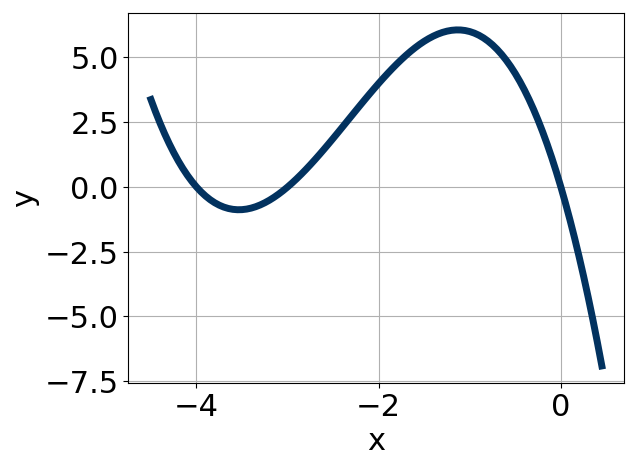
\includegraphics[width=0.5\textwidth]{../Figures/polyGraphToFunctionA.png}
\end{center}
\begin{enumerate}[label=\Alph*.]
\item \( -20(x + 1)^{8} (x + 2)^{9} (x - 3)^{11} \)
\item \( 20(x + 1)^{4} (x + 2)^{9} (x - 3)^{11} \)
\item \( 11(x + 1)^{9} (x + 2)^{10} (x - 3)^{9} \)
\item \( -3(x + 1)^{10} (x + 2)^{5} (x - 3)^{4} \)
\item \( 4(x + 1)^{4} (x + 2)^{10} (x - 3)^{5} \)

\end{enumerate} }
\end{enumerate}

\end{document}